\section{PŘESNÁ TRANZISTOROVÁ DVOJICE}
Souběh, proudové zrcadlo, diferenční stupeň, vliv rozměrů MOS tranzistorů na přesnost, Pelgromova rovnice

\subsection{Proudové zrcadlo}
\begin{figure}[h]
   \begin{center}
     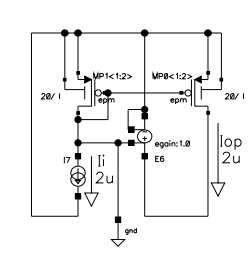
\includegraphics[scale=0.6]{images/MOS1.png}
   \end{center}
   \caption{Proudové zrcadlo}
\end{figure}

Proudové MOS zrcadlo (např. pro aktivní zátěž) navrhneme jako dvojici PMOS tranzistorů s danou šířkou kanálu W. Úkolem je poté najít takovou délku L, při níž chyba $\sigma$\textsubscript{Iop} této aktivní zátěže bude menší, než chyba vypočítaná pro diferenciální stupeň (např. 19 nA).

\begin{figure}[h]
   \begin{center}
     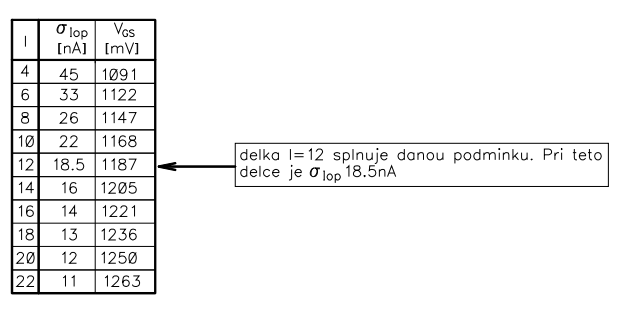
\includegraphics[scale=0.6]{images/Urceni.png}
   \end{center}
   \caption{Určení Ugs na základě chyby}
\end{figure}

\subsection{Diferenční stupeň}
\begin{figure}[h]
   \begin{center}
     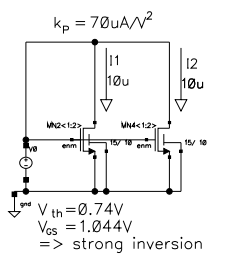
\includegraphics[scale=0.6]{images/MOS6.png}
   \end{center}
   \caption{Zapojení pro získání nesouběhu dif. stupně}
\end{figure}

Toto je základní zapojení pro měření nesouběhu dvou identických tranzistorů. Ze změřené hodnoty  chyby $\sigma$I\textsubscript{1}/I\textsubscript{2} proudu I\textsubscript{1} a I\textsubscript{2} je potom možné spočítat chybu$\sigma$\textsubscript{dVGS} souběhu V\textsubscript{GS} těchto dvou tranzistorů.
\begin{equation}
I_{2}/I_{1} = 1
\end{equation}
\begin{equation}
\sigma_{i}=\sigma_{I1/I2}*I1
\end{equation}
\begin{equation}
\sigma_{dVGS}=\frac{\sigma_{i}}{gm}
\end{equation}

Nesouběh $\sigma$\textsubscript{dVGS} dvou V\textsubscript{GS} napětí tranzistorové dvojice se projeví jako vstupní offset $\sigma$\textsubscript{VGS} elementárního operačního zesilovače.
\newpage
\subsection{Vliv rozměrů MOS tranzistorů na přesnost}
\begin{figure}[h]
   \begin{center}
     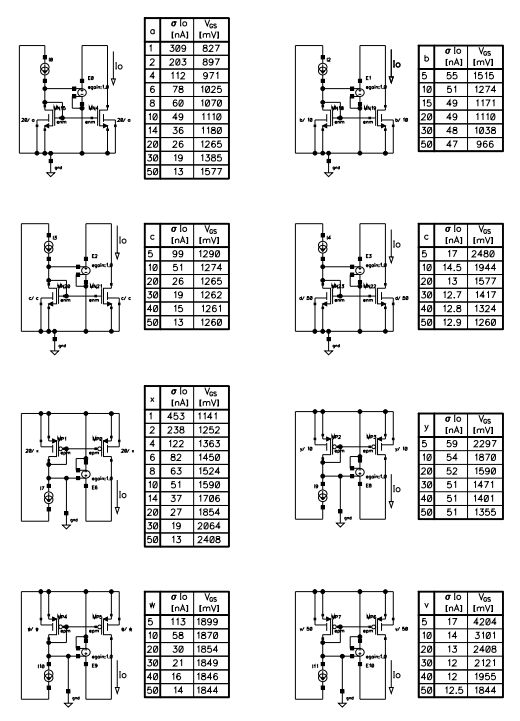
\includegraphics[scale=0.8]{images/Presnost.png}
   \end{center}
   \caption{Určení chyby na základě určení rozměrů MOS tranzistorů}
\end{figure}

\subsection{Pelgromova rovnice}
\begin{equation}
\sigma_{\Delta Id/Id}^2=\sigma_{UT0}^2*\frac{4}{(U_{GS}-U_{T0})^2}+\sigma_{\Delta \beta / \beta}^2
\end{equation}

kde chyba v U\textsubscript{T0}:
\begin{equation}
\sigma_{UT0}^2*\frac{4}{(U_{GS}-U_{T0})^2}
\end{equation}
a chyba v matchingu $\beta$:
\begin{equation}
\sigma_{\Delta \beta / \beta}^2
\end{equation}

Pro dobrý matching (malý proudový rozdíl) je dobré volit velké MOS (velké WL) a větší (U\textsubscript{GS} - U\textsubscript{T0})

\begin{figure}[h]
   \begin{center}
     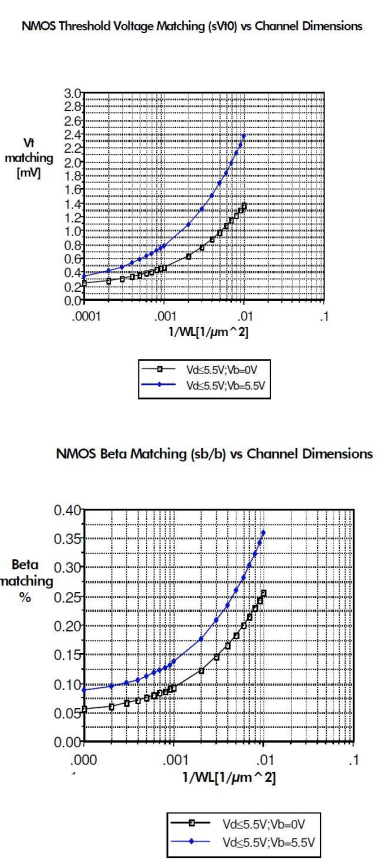
\includegraphics[scale=0.8]{images/grafy.png}
   \end{center}
   \caption{Threshold a Beta matching v závislosti na rozměrech kanálu}
\end{figure}

















